% GNUPLOT: LaTeX picture with Postscript
\begingroup
  \makeatletter
  \providecommand\color[2][]{%
    \GenericError{(gnuplot) \space\space\space\@spaces}{%
      Package color not loaded in conjunction with
      terminal option `colourtext'%
    }{See the gnuplot documentation for explanation.%
    }{Either use 'blacktext' in gnuplot or load the package
      color.sty in LaTeX.}%
    \renewcommand\color[2][]{}%
  }%
  \providecommand\includegraphics[2][]{%
    \GenericError{(gnuplot) \space\space\space\@spaces}{%
      Package graphicx or graphics not loaded%
    }{See the gnuplot documentation for explanation.%
    }{The gnuplot epslatex terminal needs graphicx.sty or graphics.sty.}%
    \renewcommand\includegraphics[2][]{}%
  }%
  \providecommand\rotatebox[2]{#2}%
  \@ifundefined{ifGPcolor}{%
    \newif\ifGPcolor
    \GPcolortrue
  }{}%
  \@ifundefined{ifGPblacktext}{%
    \newif\ifGPblacktext
    \GPblacktextfalse
  }{}%
  % define a \g@addto@macro without @ in the name:
  \let\gplgaddtomacro\g@addto@macro
  % define empty templates for all commands taking text:
  \gdef\gplbacktext{}%
  \gdef\gplfronttext{}%
  \makeatother
  \ifGPblacktext
    % no textcolor at all
    \def\colorrgb#1{}%
    \def\colorgray#1{}%
  \else
    % gray or color?
    \ifGPcolor
      \def\colorrgb#1{\color[rgb]{#1}}%
      \def\colorgray#1{\color[gray]{#1}}%
      \expandafter\def\csname LTw\endcsname{\color{white}}%
      \expandafter\def\csname LTb\endcsname{\color{black}}%
      \expandafter\def\csname LTa\endcsname{\color{black}}%
      \expandafter\def\csname LT0\endcsname{\color[rgb]{1,0,0}}%
      \expandafter\def\csname LT1\endcsname{\color[rgb]{0,1,0}}%
      \expandafter\def\csname LT2\endcsname{\color[rgb]{0,0,1}}%
      \expandafter\def\csname LT3\endcsname{\color[rgb]{1,0,1}}%
      \expandafter\def\csname LT4\endcsname{\color[rgb]{0,1,1}}%
      \expandafter\def\csname LT5\endcsname{\color[rgb]{1,1,0}}%
      \expandafter\def\csname LT6\endcsname{\color[rgb]{0,0,0}}%
      \expandafter\def\csname LT7\endcsname{\color[rgb]{1,0.3,0}}%
      \expandafter\def\csname LT8\endcsname{\color[rgb]{0.5,0.5,0.5}}%
    \else
      % gray
      \def\colorrgb#1{\color{black}}%
      \def\colorgray#1{\color[gray]{#1}}%
      \expandafter\def\csname LTw\endcsname{\color{white}}%
      \expandafter\def\csname LTb\endcsname{\color{black}}%
      \expandafter\def\csname LTa\endcsname{\color{black}}%
      \expandafter\def\csname LT0\endcsname{\color{black}}%
      \expandafter\def\csname LT1\endcsname{\color{black}}%
      \expandafter\def\csname LT2\endcsname{\color{black}}%
      \expandafter\def\csname LT3\endcsname{\color{black}}%
      \expandafter\def\csname LT4\endcsname{\color{black}}%
      \expandafter\def\csname LT5\endcsname{\color{black}}%
      \expandafter\def\csname LT6\endcsname{\color{black}}%
      \expandafter\def\csname LT7\endcsname{\color{black}}%
      \expandafter\def\csname LT8\endcsname{\color{black}}%
    \fi
  \fi
    \setlength{\unitlength}{0.0500bp}%
    \ifx\gptboxheight\undefined%
      \newlength{\gptboxheight}%
      \newlength{\gptboxwidth}%
      \newsavebox{\gptboxtext}%
    \fi%
    \setlength{\fboxrule}{0.5pt}%
    \setlength{\fboxsep}{1pt}%
\begin{picture}(10080.00,7544.00)%
    \gplgaddtomacro\gplbacktext{%
      \csname LTb\endcsname%
      \put(396,924){\makebox(0,0)[r]{\strut{}\LARGE{$0$}}}%
      \csname LTb\endcsname%
      \put(396,2094){\makebox(0,0)[r]{\strut{}\LARGE{$2000$}}}%
      \csname LTb\endcsname%
      \put(396,3264){\makebox(0,0)[r]{\strut{}\LARGE{$4000$}}}%
      \csname LTb\endcsname%
      \put(396,4433){\makebox(0,0)[r]{\strut{}\LARGE{$6000$}}}%
      \csname LTb\endcsname%
      \put(396,5603){\makebox(0,0)[r]{\strut{}\LARGE{$8000$}}}%
      \csname LTb\endcsname%
      \put(396,6773){\makebox(0,0)[r]{\strut{}\LARGE{$10000$}}}%
      \csname LTb\endcsname%
      \put(528,594){\makebox(0,0){\strut{}\LARGE{$0$}}}%
      \csname LTb\endcsname%
      \put(1639,594){\makebox(0,0){\strut{}\LARGE{$1024$}}}%
      \csname LTb\endcsname%
      \put(2749,594){\makebox(0,0){\strut{}\LARGE{$2048$}}}%
      \csname LTb\endcsname%
      \put(3860,594){\makebox(0,0){\strut{}\LARGE{$3072$}}}%
      \csname LTb\endcsname%
      \put(4970,594){\makebox(0,0){\strut{}\LARGE{$4096$}}}%
      \csname LTb\endcsname%
      \put(6081,594){\makebox(0,0){\strut{}\LARGE{$5120$}}}%
      \csname LTb\endcsname%
      \put(7191,594){\makebox(0,0){\strut{}\LARGE{$6144$}}}%
      \csname LTb\endcsname%
      \put(8302,594){\makebox(0,0){\strut{}\LARGE{$7168$}}}%
      \csname LTb\endcsname%
      \put(9412,594){\makebox(0,0){\strut{}\LARGE{$8192$}}}%
    }%
    \gplgaddtomacro\gplfronttext{%
      \csname LTb\endcsname%
      \put(-638,3848){\rotatebox{-270}{\makebox(0,0){\strut{}\LARGE{clock cycles}}}}%
      \put(5039,154){\makebox(0,0){\strut{}\LARGE{input size [bytes]}}}%
      \put(5039,7213){\makebox(0,0){\strut{}\Large{\shortstack{Data Structure Comparison on 16-bit Fixed Point Complex Multiplication\\ O3 Optimization - Average on 500000 iterations}}}}%
      \csname LTb\endcsname%
      \put(3564,6600){\makebox(0,0)[r]{\strut{}\normalsize{O3 SCALAR CMPLX STRUCT}}}%
      \csname LTb\endcsname%
      \put(3564,6380){\makebox(0,0)[r]{\strut{}\normalsize{O3 SSE4 CMPLX STRUCT}}}%
      \csname LTb\endcsname%
      \put(3564,6160){\makebox(0,0)[r]{\strut{}\normalsize{O3 AVX2 CMPLX STRUCT}}}%
      \csname LTb\endcsname%
      \put(3564,5940){\makebox(0,0)[r]{\strut{}\normalsize{O3 SCALAR CMPLX ARRAY}}}%
      \csname LTb\endcsname%
      \put(3564,5720){\makebox(0,0)[r]{\strut{}\normalsize{O3 SSE4 CMPLX ARRAY}}}%
      \csname LTb\endcsname%
      \put(3564,5500){\makebox(0,0)[r]{\strut{}\normalsize{O3 AVX2 CMPLX ARRAY}}}%
    }%
    \gplbacktext
    \put(0,0){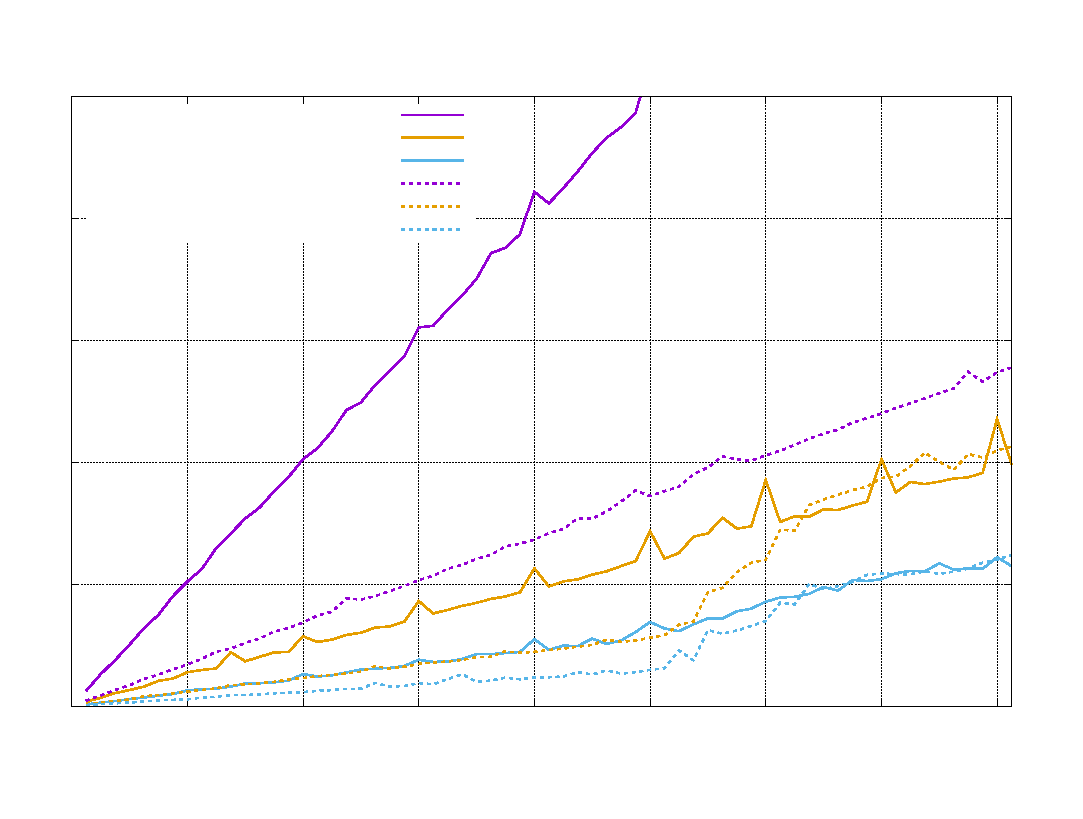
\includegraphics{complex}}%
    \gplfronttext
  \end{picture}%
\endgroup
